\documentclass[1p]{elsarticle_modified}
%\bibliographystyle{elsarticle-num}

%\usepackage[colorlinks]{hyperref}
%\usepackage{abbrmath_seonhwa} %\Abb, \Ascr, \Acal ,\Abf, \Afrak
\usepackage{amsfonts}
\usepackage{amssymb}
\usepackage{amsmath}
\usepackage{amsthm}
\usepackage{scalefnt}
\usepackage{amsbsy}
\usepackage{kotex}
\usepackage{caption}
\usepackage{subfig}
\usepackage{color}
\usepackage{graphicx}
\usepackage{xcolor} %% white, black, red, green, blue, cyan, magenta, yellow
\usepackage{float}
\usepackage{setspace}
\usepackage{hyperref}

\usepackage{tikz}
\usetikzlibrary{arrows}

\usepackage{multirow}
\usepackage{array} % fixed length table
\usepackage{hhline}

%%%%%%%%%%%%%%%%%%%%%
\makeatletter
\renewcommand*\env@matrix[1][\arraystretch]{%
	\edef\arraystretch{#1}%
	\hskip -\arraycolsep
	\let\@ifnextchar\new@ifnextchar
	\array{*\c@MaxMatrixCols c}}
\makeatother %https://tex.stackexchange.com/questions/14071/how-can-i-increase-the-line-spacing-in-a-matrix
%%%%%%%%%%%%%%%

\usepackage[normalem]{ulem}

\newcommand{\msout}[1]{\ifmmode\text{\sout{\ensuremath{#1}}}\else\sout{#1}\fi}
%SOURCE: \msout is \stkout macro in https://tex.stackexchange.com/questions/20609/strikeout-in-math-mode

\newcommand{\cancel}[1]{
	\ifmmode
	{\color{red}\msout{#1}}
	\else
	{\color{red}\sout{#1}}
	\fi
}

\newcommand{\add}[1]{
	{\color{blue}\uwave{#1}}
}

\newcommand{\replace}[2]{
	\ifmmode
	{\color{red}\msout{#1}}{\color{blue}\uwave{#2}}
	\else
	{\color{red}\sout{#1}}{\color{blue}\uwave{#2}}
	\fi
}

\newcommand{\Sol}{\mathcal{S}} %segment
\newcommand{\D}{D} %diagram
\newcommand{\A}{\mathcal{A}} %arc


%%%%%%%%%%%%%%%%%%%%%%%%%%%%%5 test

\def\sl{\operatorname{\textup{SL}}(2,\Cbb)}
\def\psl{\operatorname{\textup{PSL}}(2,\Cbb)}
\def\quan{\mkern 1mu \triangleright \mkern 1mu}

\theoremstyle{definition}
\newtheorem{thm}{Theorem}[section]
\newtheorem{prop}[thm]{Proposition}
\newtheorem{lem}[thm]{Lemma}
\newtheorem{ques}[thm]{Question}
\newtheorem{cor}[thm]{Corollary}
\newtheorem{defn}[thm]{Definition}
\newtheorem{exam}[thm]{Example}
\newtheorem{rmk}[thm]{Remark}
\newtheorem{alg}[thm]{Algorithm}

\newcommand{\I}{\sqrt{-1}}
\begin{document}

%\begin{frontmatter}
%
%\title{Boundary parabolic representations of knots up to 8 crossings}
%
%%% Group authors per affiliation:
%\author{Yunhi Cho} 
%\address{Department of Mathematics, University of Seoul, Seoul, Korea}
%\ead{yhcho@uos.ac.kr}
%
%
%\author{Seonhwa Kim} %\fnref{s_kim}}
%\address{Center for Geometry and Physics, Institute for Basic Science, Pohang, 37673, Korea}
%\ead{ryeona17@ibs.re.kr}
%
%\author{Hyuk Kim}
%\address{Department of Mathematical Sciences, Seoul National University, Seoul 08826, Korea}
%\ead{hyukkim@snu.ac.kr}
%
%\author{Seokbeom Yoon}
%\address{Department of Mathematical Sciences, Seoul National University, Seoul, 08826,  Korea}
%\ead{sbyoon15@snu.ac.kr}
%
%\begin{abstract}
%We find all boundary parabolic representation of knots up to 8 crossings.
%
%\end{abstract}
%\begin{keyword}
%    \MSC[2010] 57M25 
%\end{keyword}
%
%\end{frontmatter}

%\linenumbers
%\tableofcontents
%
\newcommand\colored[1]{\textcolor{white}{\rule[-0.35ex]{0.8em}{1.4ex}}\kern-0.8em\color{red} #1}%
%\newcommand\colored[1]{\textcolor{white}{ #1}\kern-2.17ex	\textcolor{white}{ #1}\kern-1.81ex	\textcolor{white}{ #1}\kern-2.15ex\color{red}#1	}

{\Large $\underline{12n_{0590}~(K12n_{0590})}$}

\setlength{\tabcolsep}{10pt}
\renewcommand{\arraystretch}{1.6}
\vspace{1cm}\begin{tabular}{m{100pt}>{\centering\arraybackslash}m{274pt}}
\multirow{5}{120pt}{
	\centering
	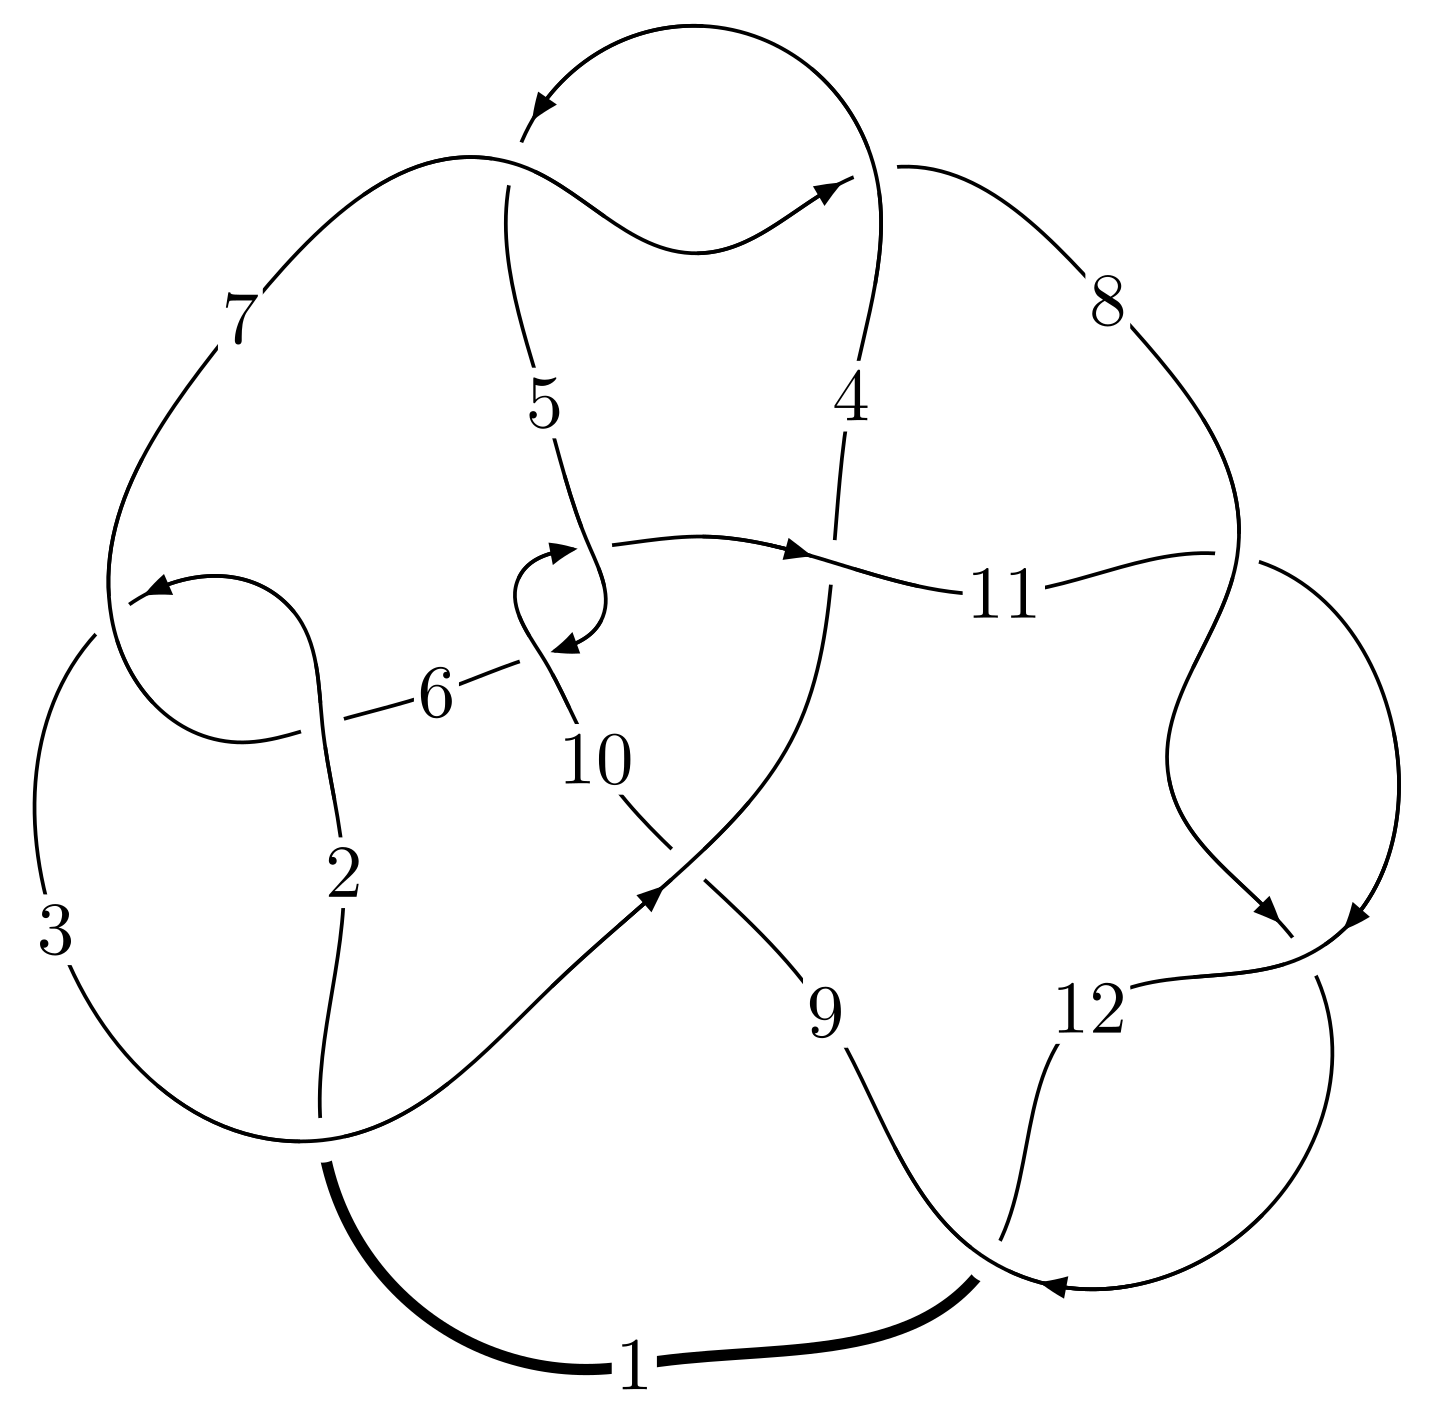
\includegraphics[width=112pt]{../../../GIT/diagram.site/Diagrams/png/2679_12n_0590.png}\\
\ \ \ A knot diagram\footnotemark}&
\allowdisplaybreaks
\textbf{Linearized knot diagam} \\
\cline{2-2}
 &
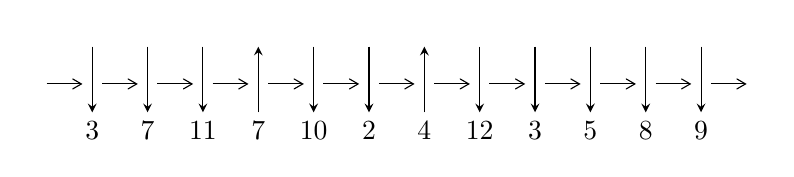
\begin{tikzpicture}[x=20pt, y=17pt]
	% nodes
	\node (C0) at (0, 0) {};
	\node (C1) at (1, 0) {};
	\node (C1U) at (1, +1) {};
	\node (C1D) at (1, -1) {3};

	\node (C2) at (2, 0) {};
	\node (C2U) at (2, +1) {};
	\node (C2D) at (2, -1) {7};

	\node (C3) at (3, 0) {};
	\node (C3U) at (3, +1) {};
	\node (C3D) at (3, -1) {11};

	\node (C4) at (4, 0) {};
	\node (C4U) at (4, +1) {};
	\node (C4D) at (4, -1) {7};

	\node (C5) at (5, 0) {};
	\node (C5U) at (5, +1) {};
	\node (C5D) at (5, -1) {10};

	\node (C6) at (6, 0) {};
	\node (C6U) at (6, +1) {};
	\node (C6D) at (6, -1) {2};

	\node (C7) at (7, 0) {};
	\node (C7U) at (7, +1) {};
	\node (C7D) at (7, -1) {4};

	\node (C8) at (8, 0) {};
	\node (C8U) at (8, +1) {};
	\node (C8D) at (8, -1) {12};

	\node (C9) at (9, 0) {};
	\node (C9U) at (9, +1) {};
	\node (C9D) at (9, -1) {3};

	\node (C10) at (10, 0) {};
	\node (C10U) at (10, +1) {};
	\node (C10D) at (10, -1) {5};

	\node (C11) at (11, 0) {};
	\node (C11U) at (11, +1) {};
	\node (C11D) at (11, -1) {8};

	\node (C12) at (12, 0) {};
	\node (C12U) at (12, +1) {};
	\node (C12D) at (12, -1) {9};
	\node (C13) at (13, 0) {};

	% arrows
	\draw[->,>={angle 60}]
	(C0) edge (C1) (C1) edge (C2) (C2) edge (C3) (C3) edge (C4) (C4) edge (C5) (C5) edge (C6) (C6) edge (C7) (C7) edge (C8) (C8) edge (C9) (C9) edge (C10) (C10) edge (C11) (C11) edge (C12) (C12) edge (C13) ;	\draw[->,>=stealth]
	(C1U) edge (C1D) (C2U) edge (C2D) (C3U) edge (C3D) (C4D) edge (C4U) (C5U) edge (C5D) (C6U) edge (C6D) (C7D) edge (C7U) (C8U) edge (C8D) (C9U) edge (C9D) (C10U) edge (C10D) (C11U) edge (C11D) (C12U) edge (C12D) ;
	\end{tikzpicture} \\
\hhline{~~} \\& 
\textbf{Solving Sequence} \\ \cline{2-2} 
 &
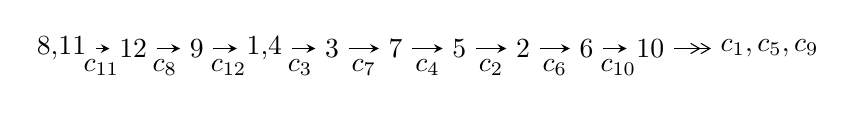
\begin{tikzpicture}[x=23pt, y=7pt]
	% node
	\node (A0) at (-1/8, 0) {8,11};
	\node (A1) at (1, 0) {12};
	\node (A2) at (2, 0) {9};
	\node (A3) at (49/16, 0) {1,4};
	\node (A4) at (33/8, 0) {3};
	\node (A5) at (41/8, 0) {7};
	\node (A6) at (49/8, 0) {5};
	\node (A7) at (57/8, 0) {2};
	\node (A8) at (65/8, 0) {6};
	\node (A9) at (73/8, 0) {10};
	\node (C1) at (1/2, -1) {$c_{11}$};
	\node (C2) at (3/2, -1) {$c_{8}$};
	\node (C3) at (5/2, -1) {$c_{12}$};
	\node (C4) at (29/8, -1) {$c_{3}$};
	\node (C5) at (37/8, -1) {$c_{7}$};
	\node (C6) at (45/8, -1) {$c_{4}$};
	\node (C7) at (53/8, -1) {$c_{2}$};
	\node (C8) at (61/8, -1) {$c_{6}$};
	\node (C9) at (69/8, -1) {$c_{10}$};
	\node (A10) at (11, 0) {$c_{1},c_{5},c_{9}$};

	% edge
	\draw[->,>=stealth]	
	(A0) edge (A1) (A1) edge (A2) (A2) edge (A3) (A3) edge (A4) (A4) edge (A5) (A5) edge (A6) (A6) edge (A7) (A7) edge (A8) (A8) edge (A9) ;
	\draw[->>,>={angle 60}]	
	(A9) edge (A10);
\end{tikzpicture} \\ 

\end{tabular} \\

\footnotetext{
The image of knot diagram is generated by the software ``\textbf{Draw programme}" developed by Andrew Bartholomew(\url{http://www.layer8.co.uk/maths/draw/index.htm\#Running-draw}), where we modified some parts for our purpose(\url{https://github.com/CATsTAILs/LinksPainter}).
}\phantom \\ \newline 
\centering \textbf{Ideals for irreducible components\footnotemark of $X_{\text{par}}$} 
 
\begin{align*}
I^u_{1}&=\langle 
24558310627155 u^{21}+76226351773367 u^{20}+\cdots+826989943797623 b-264882167921191,\\
\phantom{I^u_{1}}&\phantom{= \langle  }-1.11442\times10^{15} u^{21}-1.96283\times10^{15} u^{20}+\cdots+5.78893\times10^{15} a+1.82405\times10^{14},\;u^{22}+u^{21}+\cdots-12 u+7\rangle \\
I^u_{2}&=\langle 
- u^7+5 u^5+u^4-7 u^3-2 u^2+b+2 u,\;u^{10}-8 u^8+23 u^6- u^5-29 u^4+4 u^3+15 u^2+a-4 u-1,\\
\phantom{I^u_{2}}&\phantom{= \langle  }u^{11}-8 u^9- u^8+23 u^7+5 u^6-28 u^5-7 u^4+13 u^3+2 u^2-2 u-1\rangle \\
\\
\end{align*}
\raggedright * 2 irreducible components of $\dim_{\mathbb{C}}=0$, with total 33 representations.\\
\footnotetext{All coefficients of polynomials are rational numbers. But the coefficients are sometimes approximated in decimal forms when there is not enough margin.}
\newpage
\renewcommand{\arraystretch}{1}
\centering \section*{I. $I^u_{1}= \langle 2.46\times10^{13} u^{21}+7.62\times10^{13} u^{20}+\cdots+8.27\times10^{14} b-2.65\times10^{14},\;-1.11\times10^{15} u^{21}-1.96\times10^{15} u^{20}+\cdots+5.79\times10^{15} a+1.82\times10^{14},\;u^{22}+u^{21}+\cdots-12 u+7 \rangle$}
\flushleft \textbf{(i) Arc colorings}\\
\begin{tabular}{m{7pt} m{180pt} m{7pt} m{180pt} }
\flushright $a_{8}=$&$\begin{pmatrix}0\\u\end{pmatrix}$ \\
\flushright $a_{11}=$&$\begin{pmatrix}1\\0\end{pmatrix}$ \\
\flushright $a_{12}=$&$\begin{pmatrix}1\\u^2\end{pmatrix}$ \\
\flushright $a_{9}=$&$\begin{pmatrix}- u\\- u^3+u\end{pmatrix}$ \\
\flushright $a_{1}=$&$\begin{pmatrix}- u^2+1\\- u^4+2 u^2\end{pmatrix}$ \\
\flushright $a_{4}=$&$\begin{pmatrix}0.192509 u^{21}+0.339065 u^{20}+\cdots+1.66279 u-0.0315092\\-0.0296960 u^{21}-0.0921733 u^{20}+\cdots-0.726566 u+0.320297\end{pmatrix}$ \\
\flushright $a_{3}=$&$\begin{pmatrix}0.162813 u^{21}+0.246892 u^{20}+\cdots+0.936221 u+0.288788\\-0.0296960 u^{21}-0.0921733 u^{20}+\cdots-0.726566 u+0.320297\end{pmatrix}$ \\
\flushright $a_{7}=$&$\begin{pmatrix}-0.308808 u^{21}-0.423908 u^{20}+\cdots-4.90570 u+3.29659\\-0.0596766 u^{21}-0.0810654 u^{20}+\cdots+1.56726 u+0.227107\end{pmatrix}$ \\
\flushright $a_{5}=$&$\begin{pmatrix}-0.193496 u^{21}-0.277468 u^{20}+\cdots+1.30428 u+0.534875\\0.117215 u^{21}+0.139319 u^{20}+\cdots-0.863885 u-0.561596\end{pmatrix}$ \\
\flushright $a_{2}=$&$\begin{pmatrix}-0.340275 u^{21}-0.520418 u^{20}+\cdots-1.11925 u+4.17997\\-0.0351453 u^{21}-0.0475187 u^{20}+\cdots-0.171350 u-0.289676\end{pmatrix}$ \\
\flushright $a_{6}=$&$\begin{pmatrix}0.285354 u^{21}+0.292486 u^{20}+\cdots-3.40992 u-0.148449\\-0.0727430 u^{21}-0.200381 u^{20}+\cdots+1.21818 u+0.857957\end{pmatrix}$ \\
\flushright $a_{10}=$&$\begin{pmatrix}-0.115641 u^{21}-0.306721 u^{20}+\cdots-4.96241 u+2.03078\\0.148193 u^{21}+0.158198 u^{20}+\cdots+1.75028 u-0.764596\end{pmatrix}$\\&\end{tabular}
\flushleft \textbf{(ii) Obstruction class $= -1$}\\~\\
\flushleft \textbf{(iii) Cusp Shapes $= -\frac{5642994687059}{826989943797623} u^{21}+\frac{135118301910616}{826989943797623} u^{20}+\cdots+\frac{9106726180669764}{826989943797623} u-\frac{9982429531246890}{826989943797623}$}\\~\\
\newpage\renewcommand{\arraystretch}{1}
\flushleft \textbf{(iv) u-Polynomials at the component}\newline \\
\begin{tabular}{m{50pt}|m{274pt}}
Crossings & \hspace{64pt}u-Polynomials at each crossing \\
\hline $$\begin{aligned}c_{1}\end{aligned}$$&$\begin{aligned}
&u^{22}+44 u^{21}+\cdots+111391 u+14641
\end{aligned}$\\
\hline $$\begin{aligned}c_{2},c_{6}\end{aligned}$$&$\begin{aligned}
&u^{22}-22 u^{20}+\cdots-95 u-121
\end{aligned}$\\
\hline $$\begin{aligned}c_{3}\end{aligned}$$&$\begin{aligned}
&u^{22}+3 u^{21}+\cdots-13 u-5
\end{aligned}$\\
\hline $$\begin{aligned}c_{4},c_{7}\end{aligned}$$&$\begin{aligned}
&u^{22}+5 u^{21}+\cdots+2 u+1
\end{aligned}$\\
\hline $$\begin{aligned}c_{5},c_{10}\end{aligned}$$&$\begin{aligned}
&u^{22}- u^{21}+\cdots-123 u-173
\end{aligned}$\\
\hline $$\begin{aligned}c_{8},c_{11},c_{12}\end{aligned}$$&$\begin{aligned}
&u^{22}+u^{21}+\cdots-12 u+7
\end{aligned}$\\
\hline $$\begin{aligned}c_{9}\end{aligned}$$&$\begin{aligned}
&u^{22}-6 u^{21}+\cdots-66255 u-6691
\end{aligned}$\\
\hline
\end{tabular}\\~\\
\newpage\renewcommand{\arraystretch}{1}
\flushleft \textbf{(v) Riley Polynomials at the component}\newline \\
\begin{tabular}{m{50pt}|m{274pt}}
Crossings & \hspace{64pt}Riley Polynomials at each crossing \\
\hline $$\begin{aligned}c_{1}\end{aligned}$$&$\begin{aligned}
&y^{22}-140 y^{21}+\cdots-15971954947 y+214358881
\end{aligned}$\\
\hline $$\begin{aligned}c_{2},c_{6}\end{aligned}$$&$\begin{aligned}
&y^{22}-44 y^{21}+\cdots-111391 y+14641
\end{aligned}$\\
\hline $$\begin{aligned}c_{3}\end{aligned}$$&$\begin{aligned}
&y^{22}-3 y^{21}+\cdots-319 y+25
\end{aligned}$\\
\hline $$\begin{aligned}c_{4},c_{7}\end{aligned}$$&$\begin{aligned}
&y^{22}+21 y^{21}+\cdots-40 y+1
\end{aligned}$\\
\hline $$\begin{aligned}c_{5},c_{10}\end{aligned}$$&$\begin{aligned}
&y^{22}-9 y^{21}+\cdots-332065 y+29929
\end{aligned}$\\
\hline $$\begin{aligned}c_{8},c_{11},c_{12}\end{aligned}$$&$\begin{aligned}
&y^{22}-37 y^{21}+\cdots-186 y+49
\end{aligned}$\\
\hline $$\begin{aligned}c_{9}\end{aligned}$$&$\begin{aligned}
&y^{22}-122 y^{21}+\cdots-1381946559 y+44769481
\end{aligned}$\\
\hline
\end{tabular}\\~\\
\newpage\flushleft \textbf{(vi) Complex Volumes and Cusp Shapes}
$$\begin{array}{c|c|c}  
\text{Solutions to }I^u_{1}& \I (\text{vol} + \sqrt{-1}CS) & \text{Cusp shape}\\
 \hline 
\begin{aligned}
u &= -0.813375 + 0.695520 I \\
a &= -0.621272 + 0.888438 I \\
b &= \phantom{-}0.930849 - 0.474906 I\end{aligned}
 & -3.57261 + 1.24203 I & -13.51654 - 2.69011 I \\ \hline\begin{aligned}
u &= -0.813375 - 0.695520 I \\
a &= -0.621272 - 0.888438 I \\
b &= \phantom{-}0.930849 + 0.474906 I\end{aligned}
 & -3.57261 - 1.24203 I & -13.51654 + 2.69011 I \\ \hline\begin{aligned}
u &= \phantom{-}1.14577\phantom{ +0.000000I} \\
a &= -1.21118\phantom{ +0.000000I} \\
b &= -0.786013\phantom{ +0.000000I}\end{aligned}
 & -5.50697\phantom{ +0.000000I} & -18.3200\phantom{ +0.000000I} \\ \hline\begin{aligned}
u &= \phantom{-}0.689625 + 0.112216 I \\
a &= \phantom{-}0.60149 + 2.27758 I \\
b &= \phantom{-}0.783398 - 0.626729 I\end{aligned}
 & -2.94663 + 3.18256 I & -14.1931 - 4.5682 I \\ \hline\begin{aligned}
u &= \phantom{-}0.689625 - 0.112216 I \\
a &= \phantom{-}0.60149 - 2.27758 I \\
b &= \phantom{-}0.783398 + 0.626729 I\end{aligned}
 & -2.94663 - 3.18256 I & -14.1931 + 4.5682 I \\ \hline\begin{aligned}
u &= -1.42854 + 0.12438 I \\
a &= -0.118525 + 0.124764 I \\
b &= -0.515254 - 0.715646 I\end{aligned}
 & -3.21068 - 1.94100 I & -8.44193 + 4.49457 I \\ \hline\begin{aligned}
u &= -1.42854 - 0.12438 I \\
a &= -0.118525 - 0.124764 I \\
b &= -0.515254 + 0.715646 I\end{aligned}
 & -3.21068 + 1.94100 I & -8.44193 - 4.49457 I \\ \hline\begin{aligned}
u &= \phantom{-}0.439809 + 0.342493 I \\
a &= \phantom{-}0.658925 - 0.629517 I \\
b &= \phantom{-}0.104940 + 1.110730 I\end{aligned}
 & \phantom{-}2.79807 - 1.24078 I & -2.39806 + 5.78935 I \\ \hline\begin{aligned}
u &= \phantom{-}0.439809 - 0.342493 I \\
a &= \phantom{-}0.658925 + 0.629517 I \\
b &= \phantom{-}0.104940 - 1.110730 I\end{aligned}
 & \phantom{-}2.79807 + 1.24078 I & -2.39806 - 5.78935 I \\ \hline\begin{aligned}
u &= -1.47818 + 0.29462 I \\
a &= -0.196203 + 1.126150 I \\
b &= -0.95775 - 1.05246 I\end{aligned}
 & -10.23510 - 1.31699 I & -13.69750 + 1.12150 I\\
 \hline 
 \end{array}$$\newpage$$\begin{array}{c|c|c}  
\text{Solutions to }I^u_{1}& \I (\text{vol} + \sqrt{-1}CS) & \text{Cusp shape}\\
 \hline 
\begin{aligned}
u &= -1.47818 - 0.29462 I \\
a &= -0.196203 - 1.126150 I \\
b &= -0.95775 + 1.05246 I\end{aligned}
 & -10.23510 + 1.31699 I & -13.69750 - 1.12150 I \\ \hline\begin{aligned}
u &= -0.389548\phantom{ +0.000000I} \\
a &= \phantom{-}0.489094\phantom{ +0.000000I} \\
b &= \phantom{-}0.423427\phantom{ +0.000000I}\end{aligned}
 & -0.651086\phantom{ +0.000000I} & -15.1770\phantom{ +0.000000I} \\ \hline\begin{aligned}
u &= \phantom{-}0.055531 + 0.375870 I \\
a &= \phantom{-}3.27936 - 0.40059 I \\
b &= -0.735830 + 0.136693 I\end{aligned}
 & -1.05201 + 2.37866 I & -7.37484 + 0.30199 I \\ \hline\begin{aligned}
u &= \phantom{-}0.055531 - 0.375870 I \\
a &= \phantom{-}3.27936 + 0.40059 I \\
b &= -0.735830 - 0.136693 I\end{aligned}
 & -1.05201 - 2.37866 I & -7.37484 - 0.30199 I \\ \hline\begin{aligned}
u &= \phantom{-}1.54618 + 0.54222 I \\
a &= \phantom{-}0.045294 + 0.967197 I \\
b &= -1.17072 - 0.88115 I\end{aligned}
 & -11.07800 - 6.11809 I & -13.7689 + 3.7652 I \\ \hline\begin{aligned}
u &= \phantom{-}1.54618 - 0.54222 I \\
a &= \phantom{-}0.045294 - 0.967197 I \\
b &= -1.17072 + 0.88115 I\end{aligned}
 & -11.07800 + 6.11809 I & -13.7689 - 3.7652 I \\ \hline\begin{aligned}
u &= -1.78595\phantom{ +0.000000I} \\
a &= \phantom{-}1.55694\phantom{ +0.000000I} \\
b &= \phantom{-}0.706857\phantom{ +0.000000I}\end{aligned}
 & -16.3042\phantom{ +0.000000I} & -23.6750\phantom{ +0.000000I} \\ \hline\begin{aligned}
u &= \phantom{-}1.92376 + 0.13131 I \\
a &= -0.017132 + 0.779055 I \\
b &= \phantom{-}1.13005 - 1.28185 I\end{aligned}
 & \phantom{-}16.3680 - 1.4414 I & -13.10276 + 0.15786 I \\ \hline\begin{aligned}
u &= \phantom{-}1.92376 - 0.13131 I \\
a &= -0.017132 - 0.779055 I \\
b &= \phantom{-}1.13005 + 1.28185 I\end{aligned}
 & \phantom{-}16.3680 + 1.4414 I & -13.10276 - 0.15786 I \\ \hline\begin{aligned}
u &= -1.92464 + 0.18067 I \\
a &= \phantom{-}0.224483 + 0.973602 I \\
b &= \phantom{-}1.24119 - 1.08462 I\end{aligned}
 & \phantom{-}15.7619 + 10.2221 I & -12.91781 - 4.03002 I\\
 \hline 
 \end{array}$$\newpage$$\begin{array}{c|c|c}  
\text{Solutions to }I^u_{1}& \I (\text{vol} + \sqrt{-1}CS) & \text{Cusp shape}\\
 \hline 
\begin{aligned}
u &= -1.92464 - 0.18067 I \\
a &= \phantom{-}0.224483 - 0.973602 I \\
b &= \phantom{-}1.24119 + 1.08462 I\end{aligned}
 & \phantom{-}15.7619 - 10.2221 I & -12.91781 + 4.03002 I \\ \hline\begin{aligned}
u &= \phantom{-}2.00938\phantom{ +0.000000I} \\
a &= -0.119138\phantom{ +0.000000I} \\
b &= \phantom{-}1.03398\phantom{ +0.000000I}\end{aligned}
 & -17.7473\phantom{ +0.000000I} & -16.0060\phantom{ +0.000000I}\\
 \hline 
 \end{array}$$\newpage\newpage\renewcommand{\arraystretch}{1}
\centering \section*{II. $I^u_{2}= \langle - u^7+5 u^5+u^4-7 u^3-2 u^2+b+2 u,\;u^{10}-8 u^8+\cdots+a-1,\;u^{11}-8 u^9+\cdots-2 u-1 \rangle$}
\flushleft \textbf{(i) Arc colorings}\\
\begin{tabular}{m{7pt} m{180pt} m{7pt} m{180pt} }
\flushright $a_{8}=$&$\begin{pmatrix}0\\u\end{pmatrix}$ \\
\flushright $a_{11}=$&$\begin{pmatrix}1\\0\end{pmatrix}$ \\
\flushright $a_{12}=$&$\begin{pmatrix}1\\u^2\end{pmatrix}$ \\
\flushright $a_{9}=$&$\begin{pmatrix}- u\\- u^3+u\end{pmatrix}$ \\
\flushright $a_{1}=$&$\begin{pmatrix}- u^2+1\\- u^4+2 u^2\end{pmatrix}$ \\
\flushright $a_{4}=$&$\begin{pmatrix}- u^{10}+8 u^8-23 u^6+u^5+29 u^4-4 u^3-15 u^2+4 u+1\\u^7-5 u^5- u^4+7 u^3+2 u^2-2 u\end{pmatrix}$ \\
\flushright $a_{3}=$&$\begin{pmatrix}- u^{10}+8 u^8+u^7-23 u^6-4 u^5+28 u^4+3 u^3-13 u^2+2 u+1\\u^7-5 u^5- u^4+7 u^3+2 u^2-2 u\end{pmatrix}$ \\
\flushright $a_{7}=$&$\begin{pmatrix}- u^8- u^7+6 u^6+6 u^5-11 u^4-10 u^3+7 u^2+4 u-3\\- u^{10}+7 u^8+u^7-17 u^6-4 u^5+17 u^4+4 u^3-7 u^2+1\end{pmatrix}$ \\
\flushright $a_{5}=$&$\begin{pmatrix}u^{10}-8 u^8- u^7+23 u^6+5 u^5-28 u^4-6 u^3+14 u^2-3\\- u^{10}+7 u^8+u^7-17 u^6-4 u^5+16 u^4+4 u^3-4 u^2\end{pmatrix}$ \\
\flushright $a_{2}=$&$\begin{pmatrix}u^8+u^7-6 u^6-5 u^5+11 u^4+7 u^3-7 u^2-2 u+2\\u^7-5 u^5-2 u^4+7 u^3+5 u^2-2 u-1\end{pmatrix}$ \\
\flushright $a_{6}=$&$\begin{pmatrix}u^{10}-7 u^8- u^7+18 u^6+5 u^5-20 u^4-7 u^3+9 u^2+2 u-2\\- u^7+5 u^5+u^4-7 u^3-3 u^2+2 u+1\end{pmatrix}$ \\
\flushright $a_{10}=$&$\begin{pmatrix}u^9+u^8-6 u^7-6 u^6+11 u^5+10 u^4-7 u^3-3 u^2+3 u\\- u^3+2 u+1\end{pmatrix}$\\&\end{tabular}
\flushleft \textbf{(ii) Obstruction class $= 1$}\\~\\
\flushleft \textbf{(iii) Cusp Shapes $= 2 u^{10}-2 u^9-17 u^8+12 u^7+54 u^6-24 u^5-73 u^4+21 u^3+35 u^2-12 u-17$}\\~\\
\newpage\renewcommand{\arraystretch}{1}
\flushleft \textbf{(iv) u-Polynomials at the component}\newline \\
\begin{tabular}{m{50pt}|m{274pt}}
Crossings & \hspace{64pt}u-Polynomials at each crossing \\
\hline $$\begin{aligned}c_{1}\end{aligned}$$&$\begin{aligned}
&u^{11}-11 u^{10}+\cdots+5 u-1
\end{aligned}$\\
\hline $$\begin{aligned}c_{2}\end{aligned}$$&$\begin{aligned}
&u^{11}-3 u^{10}- u^9+8 u^8-2 u^7-10 u^6+5 u^5+6 u^4-5 u^3-2 u^2+3 u-1
\end{aligned}$\\
\hline $$\begin{aligned}c_{3}\end{aligned}$$&$\begin{aligned}
&u^{11}-2 u^{10}+3 u^9-2 u^8+u^7+u^6- u^5+u^4+5 u^3-4 u^2- u+1
\end{aligned}$\\
\hline $$\begin{aligned}c_{4}\end{aligned}$$&$\begin{aligned}
&u^{11}+3 u^9-6 u^8+u^7-20 u^6-4 u^5-26 u^4-6 u^3-15 u^2-4 u-3
\end{aligned}$\\
\hline $$\begin{aligned}c_{5}\end{aligned}$$&$\begin{aligned}
&u^{11}+4 u^9- u^8+4 u^7-4 u^6- u^5-5 u^4-2 u^3-3 u^2- u-1
\end{aligned}$\\
\hline $$\begin{aligned}c_{6}\end{aligned}$$&$\begin{aligned}
&u^{11}+3 u^{10}- u^9-8 u^8-2 u^7+10 u^6+5 u^5-6 u^4-5 u^3+2 u^2+3 u+1
\end{aligned}$\\
\hline $$\begin{aligned}c_{7}\end{aligned}$$&$\begin{aligned}
&u^{11}+3 u^9+6 u^8+u^7+20 u^6-4 u^5+26 u^4-6 u^3+15 u^2-4 u+3
\end{aligned}$\\
\hline $$\begin{aligned}c_{8}\end{aligned}$$&$\begin{aligned}
&u^{11}-8 u^9+u^8+23 u^7-5 u^6-28 u^5+7 u^4+13 u^3-2 u^2-2 u+1
\end{aligned}$\\
\hline $$\begin{aligned}c_{9}\end{aligned}$$&$\begin{aligned}
&u^{11}-5 u^{10}+\cdots+5 u-1
\end{aligned}$\\
\hline $$\begin{aligned}c_{10}\end{aligned}$$&$\begin{aligned}
&u^{11}+4 u^9+u^8+4 u^7+4 u^6- u^5+5 u^4-2 u^3+3 u^2- u+1
\end{aligned}$\\
\hline $$\begin{aligned}c_{11},c_{12}\end{aligned}$$&$\begin{aligned}
&u^{11}-8 u^9- u^8+23 u^7+5 u^6-28 u^5-7 u^4+13 u^3+2 u^2-2 u-1
\end{aligned}$\\
\hline
\end{tabular}\\~\\
\newpage\renewcommand{\arraystretch}{1}
\flushleft \textbf{(v) Riley Polynomials at the component}\newline \\
\begin{tabular}{m{50pt}|m{274pt}}
Crossings & \hspace{64pt}Riley Polynomials at each crossing \\
\hline $$\begin{aligned}c_{1}\end{aligned}$$&$\begin{aligned}
&y^{11}-31 y^{10}+\cdots-19 y-1
\end{aligned}$\\
\hline $$\begin{aligned}c_{2},c_{6}\end{aligned}$$&$\begin{aligned}
&y^{11}-11 y^{10}+\cdots+5 y-1
\end{aligned}$\\
\hline $$\begin{aligned}c_{3}\end{aligned}$$&$\begin{aligned}
&y^{11}+2 y^{10}+\cdots+9 y-1
\end{aligned}$\\
\hline $$\begin{aligned}c_{4},c_{7}\end{aligned}$$&$\begin{aligned}
&y^{11}+6 y^{10}+\cdots-74 y-9
\end{aligned}$\\
\hline $$\begin{aligned}c_{5},c_{10}\end{aligned}$$&$\begin{aligned}
&y^{11}+8 y^{10}+\cdots-5 y-1
\end{aligned}$\\
\hline $$\begin{aligned}c_{8},c_{11},c_{12}\end{aligned}$$&$\begin{aligned}
&y^{11}-16 y^{10}+\cdots+8 y-1
\end{aligned}$\\
\hline $$\begin{aligned}c_{9}\end{aligned}$$&$\begin{aligned}
&y^{11}-33 y^{10}+\cdots-11 y-1
\end{aligned}$\\
\hline
\end{tabular}\\~\\
\newpage\flushleft \textbf{(vi) Complex Volumes and Cusp Shapes}
$$\begin{array}{c|c|c}  
\text{Solutions to }I^u_{2}& \I (\text{vol} + \sqrt{-1}CS) & \text{Cusp shape}\\
 \hline 
\begin{aligned}
u &= -1.137090 + 0.296275 I \\
a &= -0.112692 - 0.807373 I \\
b &= -0.583202 - 0.143276 I\end{aligned}
 & -4.14701 - 1.11671 I & -15.2828 + 0.9622 I \\ \hline\begin{aligned}
u &= -1.137090 - 0.296275 I \\
a &= -0.112692 + 0.807373 I \\
b &= -0.583202 + 0.143276 I\end{aligned}
 & -4.14701 + 1.11671 I & -15.2828 - 0.9622 I \\ \hline\begin{aligned}
u &= \phantom{-}0.592958 + 0.265544 I \\
a &= -0.648705 - 0.517226 I \\
b &= \phantom{-}0.224636 + 1.262620 I\end{aligned}
 & \phantom{-}2.05237 - 0.90366 I & -12.99258 + 0.59002 I \\ \hline\begin{aligned}
u &= \phantom{-}0.592958 - 0.265544 I \\
a &= -0.648705 + 0.517226 I \\
b &= \phantom{-}0.224636 - 1.262620 I\end{aligned}
 & \phantom{-}2.05237 + 0.90366 I & -12.99258 - 0.59002 I \\ \hline\begin{aligned}
u &= \phantom{-}1.52480 + 0.07903 I \\
a &= -0.465943 + 0.973368 I \\
b &= -1.133880 - 0.701740 I\end{aligned}
 & -7.77644 - 4.37367 I & -13.16320 + 3.47973 I \\ \hline\begin{aligned}
u &= \phantom{-}1.52480 - 0.07903 I \\
a &= -0.465943 - 0.973368 I \\
b &= -1.133880 + 0.701740 I\end{aligned}
 & -7.77644 + 4.37367 I & -13.16320 - 3.47973 I \\ \hline\begin{aligned}
u &= -1.59014 + 0.09758 I \\
a &= \phantom{-}0.004921 - 0.710560 I \\
b &= -0.62219 + 1.27817 I\end{aligned}
 & -5.52612 + 2.32410 I & -12.39685 - 2.31746 I \\ \hline\begin{aligned}
u &= -1.59014 - 0.09758 I \\
a &= \phantom{-}0.004921 + 0.710560 I \\
b &= -0.62219 - 1.27817 I\end{aligned}
 & -5.52612 - 2.32410 I & -12.39685 + 2.31746 I \\ \hline\begin{aligned}
u &= -0.300210 + 0.263166 I \\
a &= -1.31732 + 2.93205 I \\
b &= \phantom{-}0.867895 - 0.444411 I\end{aligned}
 & -1.38510 + 3.17083 I & -10.45196 - 6.81024 I \\ \hline\begin{aligned}
u &= -0.300210 - 0.263166 I \\
a &= -1.31732 - 2.93205 I \\
b &= \phantom{-}0.867895 + 0.444411 I\end{aligned}
 & -1.38510 - 3.17083 I & -10.45196 + 6.81024 I\\
 \hline 
 \end{array}$$\newpage$$\begin{array}{c|c|c}  
\text{Solutions to }I^u_{2}& \I (\text{vol} + \sqrt{-1}CS) & \text{Cusp shape}\\
 \hline 
\begin{aligned}
u &= \phantom{-}1.81936\phantom{ +0.000000I} \\
a &= \phantom{-}1.07948\phantom{ +0.000000I} \\
b &= \phantom{-}0.493485\phantom{ +0.000000I}\end{aligned}
 & -15.7834\phantom{ +0.000000I} & -7.42530\phantom{ +0.000000I}\\
 \hline 
 \end{array}$$\newpage
\newpage\renewcommand{\arraystretch}{1}
\centering \section*{ III. u-Polynomials}
\begin{tabular}{m{50pt}|m{274pt}}
Crossings & \hspace{64pt}u-Polynomials at each crossing \\
\hline $$\begin{aligned}c_{1}\end{aligned}$$&$\begin{aligned}
&(u^{11}-11 u^{10}+\cdots+5 u-1)(u^{22}+44 u^{21}+\cdots+111391 u+14641)
\end{aligned}$\\
\hline $$\begin{aligned}c_{2}\end{aligned}$$&$\begin{aligned}
&(u^{11}-3 u^{10}- u^9+8 u^8-2 u^7-10 u^6+5 u^5+6 u^4-5 u^3-2 u^2+3 u-1)\\
&\cdot(u^{22}-22 u^{20}+\cdots-95 u-121)
\end{aligned}$\\
\hline $$\begin{aligned}c_{3}\end{aligned}$$&$\begin{aligned}
&(u^{11}-2 u^{10}+3 u^9-2 u^8+u^7+u^6- u^5+u^4+5 u^3-4 u^2- u+1)\\
&\cdot(u^{22}+3 u^{21}+\cdots-13 u-5)
\end{aligned}$\\
\hline $$\begin{aligned}c_{4}\end{aligned}$$&$\begin{aligned}
&(u^{11}+3 u^9-6 u^8+u^7-20 u^6-4 u^5-26 u^4-6 u^3-15 u^2-4 u-3)\\
&\cdot(u^{22}+5 u^{21}+\cdots+2 u+1)
\end{aligned}$\\
\hline $$\begin{aligned}c_{5}\end{aligned}$$&$\begin{aligned}
&(u^{11}+4 u^9- u^8+4 u^7-4 u^6- u^5-5 u^4-2 u^3-3 u^2- u-1)\\
&\cdot(u^{22}- u^{21}+\cdots-123 u-173)
\end{aligned}$\\
\hline $$\begin{aligned}c_{6}\end{aligned}$$&$\begin{aligned}
&(u^{11}+3 u^{10}- u^9-8 u^8-2 u^7+10 u^6+5 u^5-6 u^4-5 u^3+2 u^2+3 u+1)\\
&\cdot(u^{22}-22 u^{20}+\cdots-95 u-121)
\end{aligned}$\\
\hline $$\begin{aligned}c_{7}\end{aligned}$$&$\begin{aligned}
&(u^{11}+3 u^9+6 u^8+u^7+20 u^6-4 u^5+26 u^4-6 u^3+15 u^2-4 u+3)\\
&\cdot(u^{22}+5 u^{21}+\cdots+2 u+1)
\end{aligned}$\\
\hline $$\begin{aligned}c_{8}\end{aligned}$$&$\begin{aligned}
&(u^{11}-8 u^9+u^8+23 u^7-5 u^6-28 u^5+7 u^4+13 u^3-2 u^2-2 u+1)\\
&\cdot(u^{22}+u^{21}+\cdots-12 u+7)
\end{aligned}$\\
\hline $$\begin{aligned}c_{9}\end{aligned}$$&$\begin{aligned}
&(u^{11}-5 u^{10}+\cdots+5 u-1)(u^{22}-6 u^{21}+\cdots-66255 u-6691)
\end{aligned}$\\
\hline $$\begin{aligned}c_{10}\end{aligned}$$&$\begin{aligned}
&(u^{11}+4 u^9+u^8+4 u^7+4 u^6- u^5+5 u^4-2 u^3+3 u^2- u+1)\\
&\cdot(u^{22}- u^{21}+\cdots-123 u-173)
\end{aligned}$\\
\hline $$\begin{aligned}c_{11},c_{12}\end{aligned}$$&$\begin{aligned}
&(u^{11}-8 u^9- u^8+23 u^7+5 u^6-28 u^5-7 u^4+13 u^3+2 u^2-2 u-1)\\
&\cdot(u^{22}+u^{21}+\cdots-12 u+7)
\end{aligned}$\\
\hline
\end{tabular}\newpage\renewcommand{\arraystretch}{1}
\centering \section*{ IV. Riley Polynomials}
\begin{tabular}{m{50pt}|m{274pt}}
Crossings & \hspace{64pt}Riley Polynomials at each crossing \\
\hline $$\begin{aligned}c_{1}\end{aligned}$$&$\begin{aligned}
&(y^{11}-31 y^{10}+\cdots-19 y-1)\\
&\cdot(y^{22}-140 y^{21}+\cdots-15971954947 y+214358881)
\end{aligned}$\\
\hline $$\begin{aligned}c_{2},c_{6}\end{aligned}$$&$\begin{aligned}
&(y^{11}-11 y^{10}+\cdots+5 y-1)(y^{22}-44 y^{21}+\cdots-111391 y+14641)
\end{aligned}$\\
\hline $$\begin{aligned}c_{3}\end{aligned}$$&$\begin{aligned}
&(y^{11}+2 y^{10}+\cdots+9 y-1)(y^{22}-3 y^{21}+\cdots-319 y+25)
\end{aligned}$\\
\hline $$\begin{aligned}c_{4},c_{7}\end{aligned}$$&$\begin{aligned}
&(y^{11}+6 y^{10}+\cdots-74 y-9)(y^{22}+21 y^{21}+\cdots-40 y+1)
\end{aligned}$\\
\hline $$\begin{aligned}c_{5},c_{10}\end{aligned}$$&$\begin{aligned}
&(y^{11}+8 y^{10}+\cdots-5 y-1)(y^{22}-9 y^{21}+\cdots-332065 y+29929)
\end{aligned}$\\
\hline $$\begin{aligned}c_{8},c_{11},c_{12}\end{aligned}$$&$\begin{aligned}
&(y^{11}-16 y^{10}+\cdots+8 y-1)(y^{22}-37 y^{21}+\cdots-186 y+49)
\end{aligned}$\\
\hline $$\begin{aligned}c_{9}\end{aligned}$$&$\begin{aligned}
&(y^{11}-33 y^{10}+\cdots-11 y-1)\\
&\cdot(y^{22}-122 y^{21}+\cdots-1381946559 y+44769481)
\end{aligned}$\\
\hline
\end{tabular}
\vskip 2pc
\end{document}